\documentclass[../mech.tex]{subfiles}
\graphicspath{{\subfix{../figures/}}}
\begin{document}
\chapter{Force and Translational Dynamics}
\section{Systems and Center of Mass}
\begin{itemize}
    \item System properties are determined by the interactions between objects within the system.
    \item If the properties or interactions of the constituent objects within a system are not important in modeling the behavior of a macroscopic system, the system can itself be treated as a single object.
    \item Systems may allow interactions between constituent parts of the system and the environment, which may result in the transfer of energy or mass.
    \item For objects with symmetrical mass distributions, the center of mass is located on lines of symmetry.
    \item The location of a system's center of mass along a given axis can be calculated using the equation:
    \[ x_{cm}=\frac{\sum m_ix_i}{M}\] 
    \item For a nonuniform solid that can be considered as a collection of differential masses, $\dd m$, the solid's center of mass can be calculated using 
    \[ x_{cm}=\int x\dd m/M \]
    \item A system can be modeled as a singular object that is located at the system's center of mass.
\end{itemize}

\begin{example}
    A triangular rod of length $L$ and mass $M$ has a nonuniform linear mass density given by the equation $\lambda = \gamma x^2$ where $\gamma = \frac{3M}{L^2}$ and $x$ is the distance 
    from the left end of the rod. Determine the horizontal location of the center of the mass relative to point $P$. Express your answer in terms of $L$.

    From $\lambda =\frac{\dd m}{\dd l}$ we know that $\dd m = \lambda \dd l$. Plugging this into the center of mass formula $x_{cm}=\frac{\int \dd m}{M}$ gives us 
    $x_{cm}=\frac{\gamma \int_0^L x^3 \dd x}{M} = \frac{3}{4}L$.
\end{example}

\ex \begin{center}
    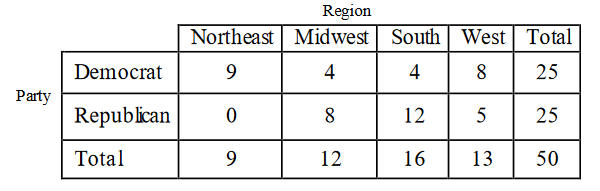
\includegraphics[width=0.5\textwidth]{2.1.1.PNG}
\end{center}
Six identical uniform spheres are arranged on a set of coordinate axes in two different triangular arrangements, $A$ and $B$, as shown. How does the $y$-coordinate of the center of mass of the 
three spheres in arrangement $A$, $y_{cm, A}$ compare to the $y$-coordinate of the center of mass of the three spheres in arrangement $B$, $y_{cm,B}$?

\pagebreak
\ex \begin{center}
    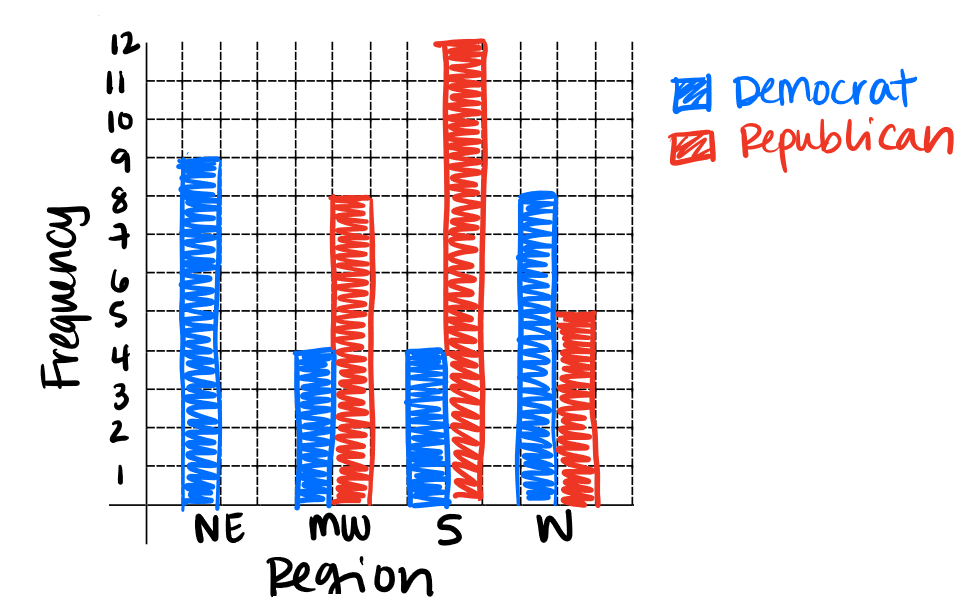
\includegraphics[width=0.5\textwidth]{2.1.2.PNG}
\end{center}
The center of mass of an irregularly shaped platform is balanced on a pivot Point $P$ with coordinates (7.0 m, 1.0 m). Two rocks are then placed on top of the platform, as shown in the top view.
One rock has a mass of 1.0 kg and is located at (-2.0 m, -3.0 m), and the second rock has a mass of 3.0 kg and is located at (5.0 m, 4.0 m). At what coordinates should a third rock of mass 4.0 kg be placed 
such that the three rock-platform system is balanced.

\section{Forces and Free-Body Diagrams}
\begin{itemize}
    \item Forces are vector quantitites that describe interactions between objects or systems.
    \item Contact forces describe the interaction of an object or system touching another object or system.
    \item Free-body diagrams (FBDs) are useful tools for visualizing forces exerted on a single object or system and for determining the equations that represent a physical situation.
    \item The FBD of an object or system shows each of the forces exerted on the object or system by the environment.
    \item Forces exerted on an object or system are represented as vector originating from the center of mass, such as a dot.
    \item Choose a coordinate system such that one axis is parallel to the acceleration of the object or system.
\end{itemize}

\begin{example}
    \begin{center}
        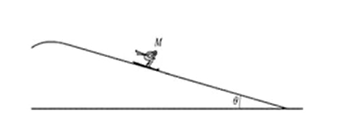
\includegraphics[width=0.5\textwidth]{2.2.PNG}
    \end{center}
    A skier of mass $M$ is skiing down a frictionless hill that makes an angle $\theta$ with the horizontal, as shown in the diagram. The skier starts from rest at time $t=0$ and is subject to a velocity-dependent drag force due to air 
    resistance of the form $F=-bv$, where $v$ is the velocity of the skier and $b$ is a positive constant. Express all algebraic answer in terms of $M, b, \theta$, and fundamental constants. Draw a dot that represents the skier, and draw a free-body
    diagram indicating and labeling all of the forces that act on the skier while the skier descends the hill.

    The correct answer will be $F_g=mg$ pointing downwards, a normal force an angle and the force $-bv$ perpendicular to this force. 
\end{example}

\pagebreak
\ex \begin{center}
    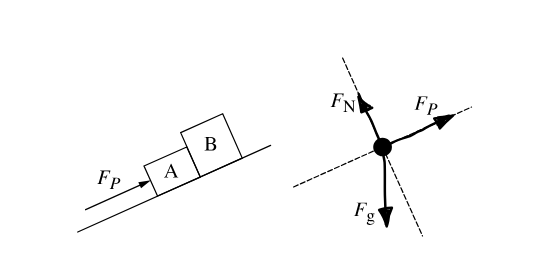
\includegraphics[width=0.5\textwidth]{2.2.1.PNG}
\end{center}
Two different blocks, $A$ and $B$, are next to each other on an inclined smooth surface which has negligible friction. An applies force, $F_P$, pushes Block $A$ as shown and the blocks move up the ramp. A student sketch of the free-body diagram representing the forces 
is given. What changes should be made to this free-body diagram?

\ex A block is at rest on a desk's horizontal surface. A student correctly identifies the force exerted on the block as the force of Earth on the block and the force of the desk on the block.
A book then is placed between the block and the desk. Which objects exert forces of equal magnitude on the block after the book has been introduced?

\section{Newton's Third Law}
Newton's third law describes the interaction of two objects or systems in terms of the paired forces that exerts on the other.
\begin{center}
    $\vec{F}_{\text{A on B}} = -\vec{F}_{\text{B on A}}$
\end{center}
Interactions between objects within a system do not influence the motion of a system's center of mass.

Tension is the macroscopic net results of forces that infinitesimal segments of a string, cable, chain or similar systme exert on each other in response to an external force.
\begin{itemize}
    \item An ideal string has negligible mass and does not stretch when under tension.
    \item The tension in an ideal string is the same at all points within the string.
    \item In a string with nonneglibible mass, tension may not be the same at all points within the string.
    \item An ideal pulley that has negligible mass and rotates about an axle through its center of mass with negligible friction.
\end{itemize}

\begin{example}
    \begin{center}
        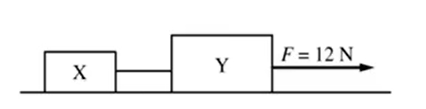
\includegraphics[width=0.5\textwidth]{2.3.PNG}
    \end{center}
    Blocks $X$ and $Y$ of masses 3.0 kg and 5.0 kg, respectively, are connected by a light string and are both on a level horizontal surface of negligible friction. A force $F=12$ N is exerted on Block $Y$, as shown in the figure above. What is the tension in the string connecting the two blocks?

    After drawing a free body diagram, we see that the $\sum F_x = ma_x$ and we can find that $a_x=1.5$ m/s$^2$.

    We alsk now that $F_T = ma_x$, so $F_T = 4.5$ N.
\end{example}

\ex A cart moving to the right collides with a stationary block, resulting in the two objects sliding together along the horizontal surface until coming to a stop.
During the collision, the cart exerts a force $F_1$ on the block, the surface exerts a force of friction $F_2$ on the block, and the block exerts a force $F_3$ on the cart. Which two forces are equal during the collision?

\ex \begin{center}
    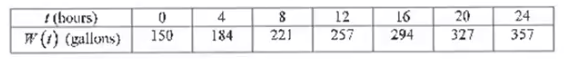
\includegraphics[width=0.5\textwidth]{2.3.1.PNG}
\end{center}
An elephant pushes two heavy boxes across a rough surface. The force that Box $A$ exerts on Box $B$ is $F_{AB}$ and the force that Box $B$ exerts on Box $A$ is $F_{BA}$. What must be true of the two boxes to support that $|F_{AB}|=|F_{BA}|$?

\section{Newton's First Law}
The net force on a system is the vector sum of all forces exerted on the system.

Translational equilibrium is the configuration of forces that the net force exerted on a system is zero.
\[ \sum F = 0 \]

Newton's first law states that if the net force exerted on a system is zero, the velocity of that system will remain constant.

Forces may be balanced in one dimension but unbalanced in another.

\begin{example}
    \begin{center}
        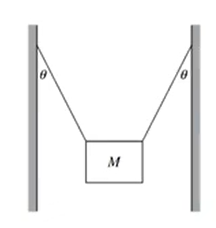
\includegraphics[width=0.5\textwidth]{2.4.PNG}
    \end{center}
    A heavy sign of mass $M$ is held at rest by two supporting wires between two buildings, with each wire making an angle $\theta$ with the vertical, as shown in the figure. What is the tension in each wire?

    Drawing the free body diagram of the system results in the following:

    In the $x$-direction, we get $T=T$.

    In the $y$-direction we get $2T\cos\theta = Mg$.

    Solving this for $T$ gives $T=\frac{Mg}{2\cos\theta}$
\end{example}

\ex An object is moving while a constant force is exerted on it. Could the addition of a force of the same magnitude cause the object to move with a constant velocity? Why or why not?

\ex \begin{center}
    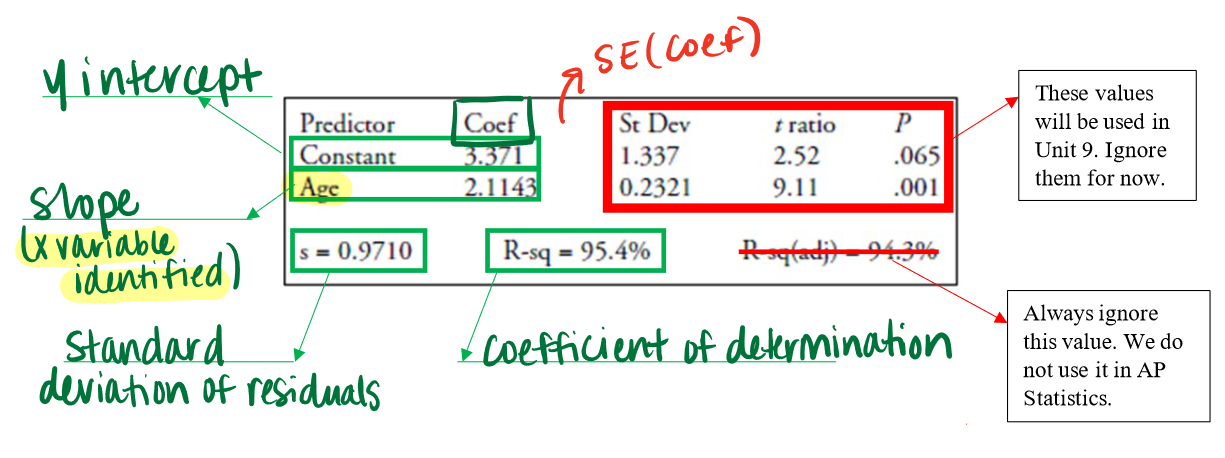
\includegraphics[width=0.5\textwidth]{2.4.1.PNG}
\end{center}
A heavy block is suspended by a string which is attached to a plastic ring. The ring is attached to two other strings which are tied to vertical supports at the angles shown. The masses of the ring and strings are negligible. 
Compare the magnitudes of the tensions in the strings $T_1$, $T_2$, and $T_3$.

\section{Newton's Second Law}
Unbalanced forces are a configuration of forces such that the net force exerted on a system is not equal to zero.

Newton's second law of motion states that the acceleration of a system's center of mass has a magnitude proportional to the magnitude of the net force exerted on the system and is in the same direction of the force.
\[ \sum F = ma =0 \]

The velocity of a system's center of mass will only change if a nonzero net external force is exerted on that system/

\begin{example}
    An object of mass 10 kg starts from rest at time $t=0$ and moves in a straight line. For time $t>0$, the object's velocity as a function of time $t$ is given by $v=2t+3t^2$, where $v$ is in m/s and $t$ is in seconds. What is the instantaneous net force that acts on the object at $t=2$ s?

    The acceleration function is given by $2+6t$, so $a(2)=14$ m/s$^2$.

    $F=ma$, so plugging in numbers gives 140 N.
\end{example}

\ex \begin{center}
    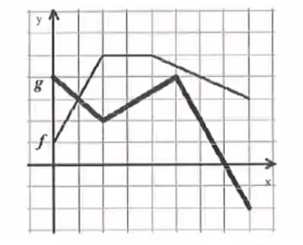
\includegraphics[width=0.5\textwidth]{2.5.1.PNG}
\end{center}
Three large blocks, $A$, $B$, and $C$, and a small block attached to Block $B$ slide across a horizontal surface as a constant force $F$ is exerted on Block $A$, as shown in the figure.
There is negligible friction between the blocks and the horizontal surface. Block $A$ pushes Block $B$ with a force $F_{AB}$. The small block is then removed from Block $B$ and attached to Block $C$ and the same force $F$ 
is exerted on Block $A$. How does $F_{AB}$ compare in the second situation to the first situation and why?

\pagebreak
\ex \begin{center}
    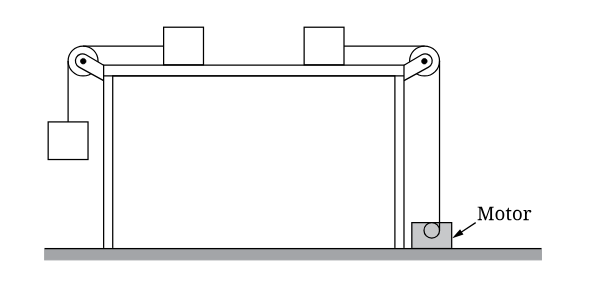
\includegraphics[width=0.5\textwidth]{2.5.2.PNG}
\end{center}
Two identical blocks are placed on a table as shown in the figure. The block on the left is attached to another identical block hanging over the edge of the table. The block on the right is attached to a motor pulling downward 
with a constant tension equal to the weight of one block. The mass of the strings and friction between the blocks and table are negligible and the pulleys are ideal. How do the magnitudes of the acceleration of the blocks compare and why?

\section{Gravitational Force}
Newton's law of universal gravitation describes the gravitational force between two objects as directly proportional to each of their masses and inversely proportional to the square of the distance between their centers.
\[ F_G = \frac{Gm_1m_2}{d^2} \]

A field models the effects of a noncontact force exerted on an object at various positions in space.

The magnitude of the gravitational field created by a system of mass $M$ at a point in space is equal to the ratio of the gravitational force exerted by the system on a test object of mass $m$ to the mass of the test object. 
\[ \vec{g}=\frac{\vec{F}_g}{m} \]

If a system is accelerating, the apparent weight of the system is not equal to the magnitude of the gravitational force exerted on the system.

Newton's shell law theorem describes the net gravitational force exerted on an object by a uniform spherical shell of mass.

\begin{example}
    \begin{center}
        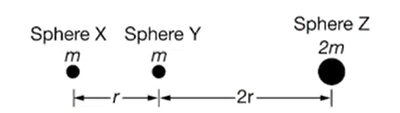
\includegraphics[width=0.5\textwidth]{2.6.PNG}
    \end{center}
    Spheres $X$, $Y$, and $Z$ have the masses and locations indicated in the figure above. What is the magnitude of the net gravitational force on sphere $X$ due to the other two spheres?

    We have that $F_y=\frac{Gm^2}{r^2}$ and $F_z= \frac{1}{2}\frac{Gm^2}{r^2}$ so adding these two together gives $\frac{3}{2}\frac{Gm^2}{r^2}$.
\end{example}

\pagebreak
\ex \begin{center}
    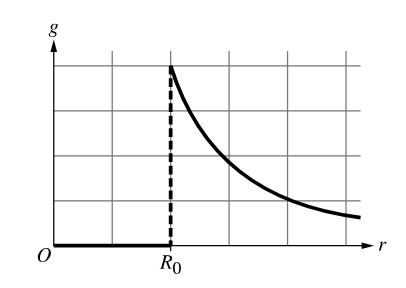
\includegraphics[width=0.5\textwidth]{2.6.1.PNG}
\end{center}
The gravitational field $g$ of a spherically symmetric object of radius $R_0$ as a function of distance $r$ from the object's center is shown in the graph. What best describes the object?

\ex \begin{center}
    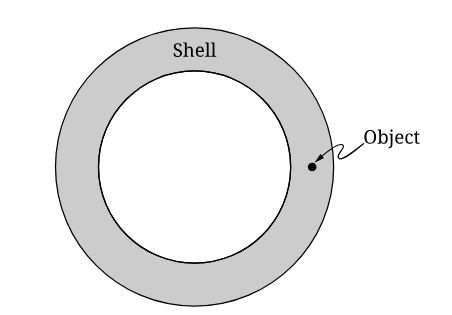
\includegraphics[width=0.5\textwidth]{2.6.2.PNG}
\end{center}
A large spherical shell with a uniform mass distribution contains a small object within the thickness of the shell, as shown in the figure. At which locations could the object be moved to increase the magnitude of the gravitational force exerted on the object by the shell?

\section{Kinetic and Static Friction}
Kinetic friction occurs when two surfaces in contact move relative to each other.
\begin{itemize}
    \item It opposes the direction of motion.
    \item The surface area of contact is not a factor.
\end{itemize}

The magnitude of the kinetic friction force exerted on an object is the product of the normal force the surface exerts on the object and the coefficient of kinetic friction.
\[ f_k = \mu_k F_N \]

Static friction may occur between the contacting surfaces of two objects that are not moving relative to each other.

Static friction adopts the value and direction required to prevent an object from slipping or sliding on a surface.
\[ f_s \leq \mu_s F_N \]

The coefficient of static friction is typically greater than the coefficient of kinetic friction for a given pair of surfaces.

\begin{example}
    \begin{center}
        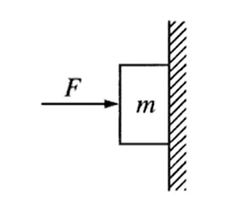
\includegraphics[width=0.5\textwidth]{2.7.PNG}
    \end{center}
    A horizontal force $F$ pushes a block of mass $m$ against a vertical wall. The coefficient of friction between the block and the wall is $\mu$. What value of $F$ is necessary to keep the block from slipping down the wall?

    In the $x$ direction the forces result in $F_N=F$.

    In the $y$ direction the forces end up with $f=F_g$ or $\mu F_N= mg = \mu F = mg$. The force is therefore $F=\frac{mg}{\mu}$.
\end{example}

\ex \begin{center}
    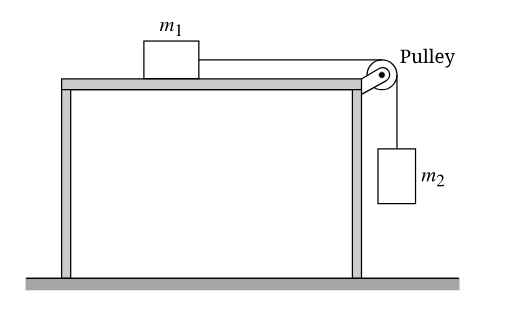
\includegraphics[width=0.5\textwidth]{2.7.1.PNG}
\end{center}
A block of mass $m_1$ rests on a rough horizontal tabletop, as shown in the figure. The block is connected by a string to a second block of mass $m_2$, which hangs below a pulley at the edge of the table.
The coefficient of static friction between the tabletop and the first block is $\mu_s$. The masses of the string and the pulley are negligible, and the pulley can rotate with negligible friction on its axle.
What is the minimum mass $m_2$ that will cause the blocks to start moving?

\ex A rectangular block is pushed by a constant force and accelerates along a rough horizontal surface. The block can be oriented to slide along any of three different sides, $A$, $B$, and $C$. Sides $A$, $B$, and $C$ have surface areas 
$S_A$, $S_B$, and $S_C$, respectively where $S_A<S_B<S_C$. On which side should the block be placed to have the greatest magnitude of acceleration?

\section{Spring Forces}
An ideal spring has negligible mass and exerts a force that is proportional to the change in its length as measured from its relaxed length.

The magnitude of the force exerted by an ideal spring on an object is given by Hooke's Law:
\[ F_{sp}=-k\Delta x \] 

The force exerted on an object by a spring is always directed toward the equilibrium position of the object-spring system.

A collection of springs that exert forces on an object may behave as though they were a single spring with an equivalent spring constant.
\begin{itemize}
    \item Springs in series: $\frac{1}{k_{eff}}=\frac{1}{k_1}+\frac{1}{k_2}+\dots$
    \item Springs in parallel: $k_{eff}=k_1+k_2+\dots$
\end{itemize}

\begin{example}
    To illustrate a human soft tissue deformation, a science teacher uses two ideal springs and a small sphere. The sphere of mass $m_s$ is attached to the free ends of the two springs. Then, the system is 
    suspended vertically. The upper string has an equilibrium $L_u$ and a spring constant $k_u$. The lower spring has an equilibrium length $L_l$ and a spring constant $k_l$. The teacher fixes an additional small block of mass 
    $m_b$ to the free end of the lower spring. Find the expression of the system's total length.

    The upper string is given as $F_{sp}=k_u\Delta x_u$. Plugging in total mass and gravity we get $(m_b+m_s)g=k_u\Delta x_u$. Solving for $\Delta x_u$ gives $\Delta x_u = \frac{(m_b+m_s)g}{k_u}$

    The lower string is given by a similar approach and gives us $\Delta x_l=\frac{m_b g}{k_l}$.

    The total length is therefore $L_T = L_l + L_u + \frac{(m_b+m_s)g}{k_u}+\frac{m_b g}{k_l}$.
\end{example}

\ex When a block of mass $M$ is hung vertically from a spring, the spring is stretched by a distance $D$ compared to its unstretched length. If a second identical spring is connected in series with the first spring and a larger 
block of mass $2M$ is then hung vertically from the two-spring combination, by how much is the combination stretched compared to its unstretched length?

\ex \begin{center}
    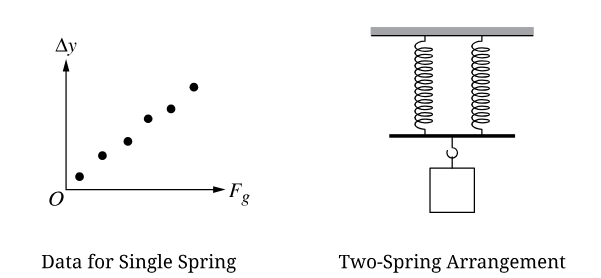
\includegraphics[width=0.5\textwidth]{2.8.PNG}
\end{center}
Some students attach a single spring to a clamp and let the spring hang vertically. Objects of different mass are attached to the free end of the spring and allowed to hang at rest. The students measure the 
distance $\Delta y$ the spring stretches from its equilibrium length for each object. The students produce the graph of $\Delta y$ as a function of the weight $F_g$ of the objects shown in the figure, and the slope of the best-fit line to the data is determined to be 
$S_1$. Next, the students take a second spring that is identical to the first and arrange the two springs as shown in the two-spring arrangement next to the graph. Once again, the objects of different mass are attached to the two-spring arrangement,
$\Delta y$ is measured, and the data is plotted on another graph showing $\Delta y$ as a function of $F_g$. What best describes the slope of the best-fit line to the data collected for the two-spring arrangement?

\section{Resistive Forces}
A resistive force is defined as a velocity-dependent force in the opposite direction of an object's velocity.
\[ F_R=-kv [F_R=-bv^2] \]

Applying Newton's second law to an object upon which a resistive force is exerted results in a differential equation for velocity.
\begin{itemize}
    \item The differential portion of a=the equation comes from substituting in $a=\frac{\dd v}{\dd t}$
\end{itemize}

Terminal velocity is defined as the maximum speed achieved by an object moving under the influence of a constant force and a resistive force that are exerted on the object in opposite directions.
\begin{itemize}
    \item For a falling object, this occurs when the air resistance equals the weight of the object.
\end{itemize}

\begin{example}
    \begin{center}
        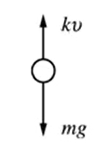
\includegraphics[width=0.5\textwidth]{2.9.PNG}
    \end{center}
    The object of mass $m$ shown above is dropped from rest near Earth's surface and experiences a resistive force of magnitude $kv$, where $v$ is the speed of the object and $k$ is a constant. Derive an expression for the velocity of the object at any point in time. (Assume that the direction of the gravitational force is positive.)

    We have that $\Delta F = ma$ so we have $mg-kv=ma$. We also have $mg-kv=m\frac{\dd v}{\dd t}$ as well as $mg-kv_T=0$, so $v_T = \frac{mg}{k}$.

    From $mg-kv=m\frac{\dd v}{\dd t}$ we can simplify this to $\int_0^t \dd t = \int_0^{v(t)} \frac{\dd v}{g-\frac{kv}{m}}$.

    Solving this gives $t=-\frac{m}{k}\ln(1-\frac{kv}{mg})$.

    Simplifying for $v(t)$ gives $v(t)= \frac{mg}{k}\left(1-e^{-\frac{kt}{m}}\right)$.
\end{example}

\ex An object is released from rest and falls to the ground near Earth's surface. The resistive force exerted on the object is directly proportional to the speed of the object which results 
in a velocity function which includes the term $e^{-\frac{t}{\beta}}$, where $\beta$ is a positive constant. What best describes the motion of the object if it falls for a time equal to $\beta$?

\ex Two spheres, $A$ and $B$, of identical size and surface material, but different masses, are dropped from rest near the surface of Earth. While falling, each sphere experiences a resistive force which is proportional 
to the sphere's velocity. What are the relationships of the magnitude of the initial acceleration $a_0$ of each sphere and of the terminal speed $v_T$ of each sphere if $m_A<m_B$?

\section{Circular Motion}
Centripetal acceleration is the component of an object's acceleration directed toward the center of the object's circular path.
\begin{itemize}
    \item The magnitude of the acceleration for an object moving in a circular path is the ratio of the object's tangential speed squared to the radius of the circular path.
    \[ a_c=v^2/r \]
\end{itemize}
Centripetal acceleration can result from a single force, more than one force, or components of forces that are exerted on an object in circular motion.

Tangential acceleration is the rate at which an object's speed changes and is directed tangent to the object's circular path. 
\[a=\sqrt{a_c^2+a_T^2}\]

The net acceleration of an object moving in a circle is the vector sum of the centripetal acceleration and tangential acceleration.

The revolution of an object traveling in a circular path at a constant speed (UCM) can be described using period and frequency.
\[v=\frac{2\pi r}{T}=2\pi r f \qquad T=\frac{1}{f}\]

\begin{example}
    A billiard ball (mass $m=0.150$ kg) is attached to a light string that is 0.50 meters long and swung so that it travels in a horizontal, circular path of radius 0.40 m, as shown.
    \begin{center}
        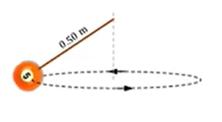
\includegraphics[width=0.5\textwidth]{2.10.PNG}
    \end{center}

    a. On the diagram, draw a free-body diagram of the forces acting on the billiard ball.    

    There will be a force $T$ in the direction of the string, $a_c$ pointing right from the billiard ball and $F_g$ pointing downwards.

    b. Calculate the force of tension in the string as the ball swings in a horizontal circle.

    We know that $T\sin\theta = F_g$. From this we can determine that $T=2.5$ N.

    c. Determine the magnitude of the centripetal acceleration of the ball as it travels in the horizontal circle.

    We know that $T\cos\theta = ma_c$, so solving for $a_c$ gives us 13.3 m/s$^2$.

    d. Calculate the period $T$ (time for one revolution) of the ball's motion. 

    We know that $a_c=\frac{v^2}{r}$ so we can find that that $v$ = 2.30 m/s. We also know that $v=\frac{2\pi r}{T}$, so solving for $T$ gives 1.15.
\end{example}
\ex An object of mass $m$ is attached to the end of a spring. The string is spun around in a vertical circle of radius $r$. When the object is at the top of its path, the speed of the object is $v$ and the string has a tension $F_T$. Write an expression for $v$ at the top of the circular path.

\ex Two small blocks, $P$ and $Q$ rotate without slipping on a horizontal disk with Block $P$ being twice as far from the rotational axis of the disk as Block $Q$. The blocks are made of the same material and Block $P$ is half the mass of Block $Q$. As the disk increases in speed, which block will be the first to begin to slide on the disk's surface?

\end{document}